\documentclass[11pt]{IEEEtran}

\usepackage{cite, multicol, float}
\usepackage{gensymb, amssymb, amsmath}
\usepackage{graphicx}
\usepackage{stfloats}

\usepackage[margin=1in]{geometry}
\usepackage[font=scriptsize,labelfont=bf]{caption}
\usepackage{setspace}
\setlength{\parskip}{0pt}

\usepackage{enumitem}
\setlist{topsep=11pt}

%\doublespacing
\onehalfspacing

\begin{document}


% Turn off two column)
\twocolumn[ \begin{@twocolumnfalse}
		
% Title
\title{Spiral Packing}
\author{Adrian Cortez \\
	Rochester Institute of Technology \\
	\small \texttt{arc6210@rit.edu}}
\date{May 2015}
\maketitle
	
% Abstract	
\begin{abstract}
Cameron Browne and Paul van Wamelen present a simple iterative method for creating artistic, space-filling designs based on spiral packings, utilizing circle approximations to significantly simplify the spiral packing problem.\cite{Browne2006834} In this paper we implement the algorithm described by Browne and van Wamelen, discuss the underlying geometry in detail and provide a number of color examples generated by the algorithm. The resulting images are evaluated based on how well they are packed and on aspects of their overall design. We show that the algorithm provides a good approximation and generates designs that are both space-filling and visually pleasing.
\break \break
\end{abstract}

\end{@twocolumnfalse}]


% Introduction
\section{Introduction}
Spiral packing is the process of filling a given area, or shape boundary, with connected sets of spirals. The sets are generated by successively branching child spirals from parent spirals, constrained to fit nearby neighbors in their environment. This process continues until the area is filled to some desired level of coverage. The ultimate goal is to generate designs that are artistic and space-filling. Examples of generated images using the spiral packing algorithm are shown in Figure~\ref{fig:example}.

\begin{figure}[h]
\centering 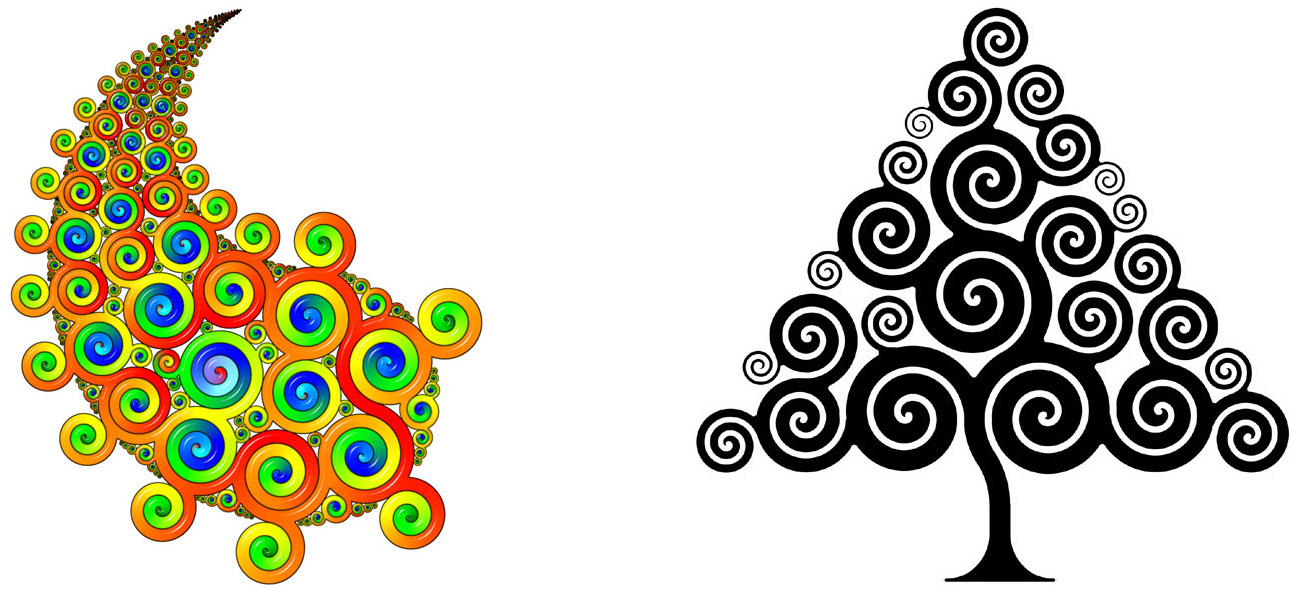
\includegraphics[width=0.9\linewidth]{spiral-packing-example}
\caption{Examples of spiral packing. \cite{Browne2006834}}
\label{fig:example}
\end{figure}


\subsection{Archimedes' Spiral}	
The general polar equation for the Archimedean spiral is 
\begin{equation} 
\label{eq:1} 
	r(\theta) = a\theta^\frac{1}{n} 
\end{equation}

The implemented algorithm utilizes the special case of the Archimedean spiral (\begin{math}n=1\end{math}), known as Archimedes' spiral (Figure~\ref{fig:spiral}, left), described by the equation \begin{math} r = a\theta \end{math}. This special case was chosen by the authors because of its aesthetic and well-behaved mathematical qualities.\cite{Browne2006834}
	
\begin{figure}[h]
\centering
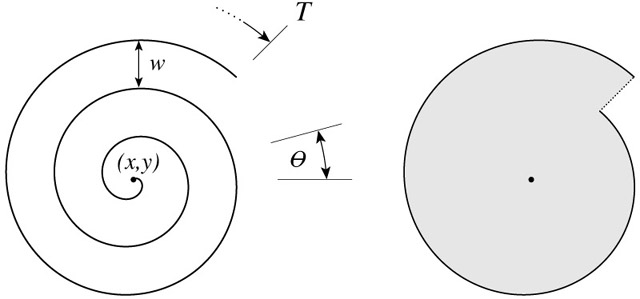
\includegraphics[width=0.9\linewidth]{spiral-packing-fig-02}
\caption{Archimedes's spiral and its footprint. \cite{Browne2006834}}
\label{fig:spiral}
\end{figure}

\begin{figure*}[b!]
\centering
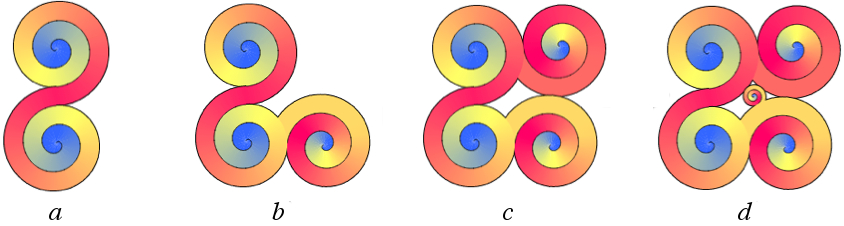
\includegraphics[width=0.75\textwidth]{spiral-branching}
\caption{A simple example of the packing process. The process starts with a pair of seed spirals. Child spirals are then successively branched from the parent spirals, fitting to any potentially intersecting neighbors.}
\label{fig:branch}
\end{figure*}

The Archimedes' spiral can be described in cartesian coordinates by the set of parameters \begin{math}(x,y,w,\theta,T,\omega)\end{math}, giving the parametric equations:
\begin{equation} 
\label{eq:2} 
	x_{s}(t) = x + wt cos(\theta + 2\pi\omega t)
\end{equation}
\begin{equation}
\label{eq:3} 
	y_{s}(t) = y + wt sin(\theta + 2\pi\omega t) 
\end{equation}
for \begin{math}0 \leq t \leq T\end{math}, where \begin{math}(x,y)\end{math} is the spiral's center, \begin{math}w\end{math} is the width of one rotation, \begin{math}\theta\end{math} is the starting angle or phase, \begin{math}T\end{math} is the number of rotations or total sweep of the spiral, and \begin{math}\omega\end{math} is the orientation of the spiral (\begin{math}\omega = -1\end{math} for clockwise and \begin{math}\omega = 1\end{math} for counterclockwise).

The area enclosed by the outer 360\degree\ sweep of a spiral is described as its footprint (Figure~\ref{fig:spiral}, right). The equation for finding the area bounded by a curve in polar coordinates is 
\begin{equation} \label{eq:4}
	A_{s} = \frac{1}{2} \int_{a}^{b} r(\theta)^2 d\theta
\end{equation}
By using the polar form of the spiral (equation \ref{eq:1}) with \begin{math} n = 1 \end{math} and \begin{math} a = \frac{w}{2 \pi} \end{math} we can calculate the area of the footprint, and therefore the area of the spiral, as
\begin{equation} 
\label{eq:5} 
\begin{split}
	A_{s} &= \frac{1}{2} \int_{2 \pi (T-1)}^{2 \pi T} (a\theta)^2 d\theta \\
		 &= \frac{4 \pi^3 a^2}{3} (T^3 - (T-1)^3) \\
		 &= \frac{\pi w^2}{3} (T^3 - (T-1)^3) 
\end{split} 
\end{equation}
Notice that the bounds of the integral span from from \begin{math} T-1 \end{math} to \begin{math} T \end{math}, corresponding to the outer turn of the spiral. This is necessary to avoid counting some regions of the spiral area multiple times.

\subsection{Spiral Packing}
The goal is to pack a given area with connected sets of Archimedes' spirals. The packing process begins with one or more pairs of seed spirals from which child spirals are successively branched. The seed spirals are generated as a pair of opposed matching spirals, \begin{math}S_{1}\end{math} and \begin{math}S_{2}\end{math}. The seed spirals have identical \begin{math} w, T, \omega \end{math}, opposed \begin{math}\theta\end{math} and are oriented with tangential endpoints such that \begin{math} x_{s_{1}}(T) = x_{s_{2}}(T-1) \end{math}, 
\begin{math} y_{s_{1}}(T) = y_{s_{2}}(T-1)\end{math}, 
\begin{math} x_{s_{1}}(T-1) = x_{s_{2}}(T)\end{math}, and 
\begin{math} y_{s_{1}}(T-1) = y_{s_{2}}(T) \end{math}. 
This relationship is shown in Figure~\ref{fig:branch}a. This process continues by branching child spirals from parent spirals until the target area is packed to some desired density. 

The term \textit{connected spiral set} is used to describe the collection of spirals that ultimately branch from a single seed pair. This means that there will be as many spiral sets as there are seed pairs. The defining property of connected spiral sets is that every interior point within the set is connected to every other. When generating connected spiral sets, the following constraints must not be violated:
\begin{enumerate}
  \item A child must have only one parent, though parents may have multiple children,
  \item A child must not have a greater width \begin{math}w\end{math} than its parent,
  \item Each child must meet its parent tangentially,
  \item Each child must be rotated such that its terminal point lies on the line drawn between its center and its parent's center, and
  \item Spirals may touch neighboring spirals tangentially but may not intersect them.
\end{enumerate}

Figure~\ref{fig:branch} demonstrates a simple example of the packing process. The process starts with a seed pair (Fig.~\ref{fig:branch}a) from which a single spiral branches (Fig.~\ref{fig:branch}b). Then an additional spiral is branched, touching one other spiral tangentially (Fig.~\ref{fig:branch}c). A final spiral is then placed, its width constrained (lessened) so that it touches the two neighboring spirals without intersecting them (Fig.~\ref{fig:branch}d).

\begin{figure*}[t]
\centering 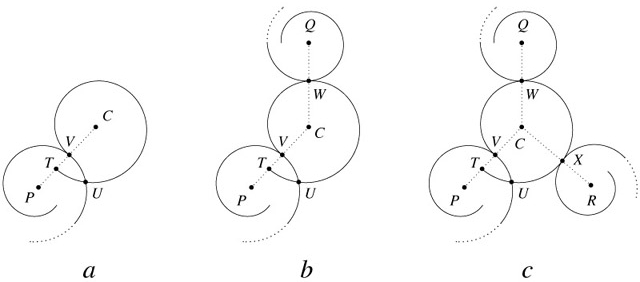
\includegraphics[width=0.55\textwidth]{spiral-packing-fig-01}
\caption{The three geometric cases when branching: (a) simple branching, (b) fitting a child spiral to one neighboring spiral, and (c) fitting a child spiral to two neighboring spirals. \cite{Browne2006834}}
\label{fig:geo}
\end{figure*}

The underlying geometry that captures these constraints can be described in three general cases, as shown in Figure~\ref{fig:geo}. 

\begin{enumerate}
\item \textit{Case I}: The most simple branching case. A child spiral \begin{math}S\end{math}, branching from an existing parent spiral \begin{math}S_{1}\end{math}, is placed in such a way that it does not intersect any neighboring spirals (Fig~\ref{fig:geo}a). This is handled simply by drawing \begin{math}S\end{math} at the specified location. 
\item \textit{Case II}: A child spiral \begin{math}S\end{math}, branching from an existing parent spiral \begin{math}S_{1}\end{math}, is placed so that it intersects one neighboring spiral, \begin{math}S_{2}\end{math} (Fig~\ref{fig:geo}b). \begin{math}S\end{math} must be repositioned, resized, or both so that it lies tangent to \begin{math}S_{2}\end{math}.
\item \textit{Case III}: A child spiral \begin{math}S\end{math}, branching from an existing parent spiral \begin{math}S_{1}\end{math}, is placed so that it intersects two neighboring spirals, \begin{math}S_{2}\end{math} and  \begin{math}S_{3}\end{math} (Fig~\ref{fig:geo}c). \begin{math}S\end{math} must be repositioned, resized, or both so that it lies tangent to both \begin{math}S_{2}\end{math} and  \begin{math}S_{3}\end{math}. 
\end{enumerate}

In the case where two neighboring spirals are intersected, there is a possibility that the algorithm may not converge in a way to allow the child spiral to lie tangent to both neighbors. In this case, the maximally intersected neighbor is chosen as the spiral to position the child spiral tangent to.

In all cases, the child spiral \begin{math}S\end{math} is rotated to lie tangent to the parent spiral \begin{math}S_{1}\end{math} such that its end point \begin{math}T\end{math} lies on the line between the spiral centers. \begin{math}S\end{math} is clipped at the intersection point \begin{math}U\end{math} and \begin{math}S_{1}\end{math} is clipped along the interval between the tangent point \begin{math}V\end{math} and intersection point \begin{math}U\end{math}. Following clipping, there should be no intersection between any pair of spirals within the packing. The parent spiral is considered a complete spiral even though intervals along its sweep may be clipped by children.

\subsection{Apollonian Packing}	
In the 3rd century BC the Greek geometer Apollonius of Perga described the class of problems of drawing a circle tangent to three other objects. Each of these objects could be either a point, line or circle. There are a total of ten different cases, collectively known as circle packing or Apollonian packing.\cite{Bourke2006}

For the purposes of simplifying the spiral packing process, we are interested only in the solution to the last of the ten cases; the problem of fitting a circle tangent to three other circles, known as Apollonius' Tenth problem (Figure~\ref{fig:circle}) . In particular, we are interested in the solution that yields the minimum radius.\cite{Browne2006834} By approximating the spirals as circles the spiral packing problem is reduced to the circle packing problem of interest. This significantly simplifies the process of fitting a child spiral to neighboring spirals.

\begin{figure}[H]
\centering 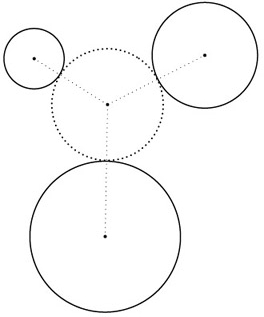
\includegraphics[width=33.3mm, height=40mm]{spiral-circles}
\caption{An example Apollonian packing for the case of one circle fitting tangent to three other circles.\cite{Browne2006834}}
\label{fig:circle}
\end{figure}

There are obvious similarities between the packing of circles and the packing of spirals. However, there are differences that make spiral packing a more difficult problem to solve. With that said, the solution to the circle packing problem provides a good framework on which to build a robust approximate solution to achieve the spiral packing that is desired.\cite{Browne2006834}.


% Implementation
\section{Implementation}
To begin the generation of the connected spiral sets, the implemented program starts with one or more pairs of seed spirals from which the child spirals can branch. During the branching process, the user will need to provide a preferred location for the child spirals. The algorithm will take this preferred location in conjunction with the constraints listed above and the state of the packed area to attempt to place the child spiral. The goal is to place the child spiral as close to the user's preferred location as possible without violating the constraints.

% Results
\section{Results}
The results of the algorithm will be evaluated in two ways. The first evaluation technique is purely visual; the algorithm must produce images that are aesthetically pleasing as well as space-filling. This is determined not only by the generated connected spiral sets adhering to the constraints listed above, but also by the coloring of the resulting images. In order to properly evaluate the robustness of the implementation, several images will be generated to demonstrate different packing scenarios, bounding areas, arrangements, and color schemes. The second way of evaluating the results is by calculating the \textit{porosity}, or the ratio of vacant area to the area covered by spirals. The lower the porosity, the better the packing. For the purposes of this project, a porosity of 5\% or lower will be considered a good packing. 

\subsection{Evaluation}


% Conclusion
\section{Conclusion}


% References
\bibliographystyle{plain}
\bibliography{references}{}

\end{document}